%\documentclass{book}\usepackage{sjtfonts}\usepackage{includegraphics}\usepackage{alltt}\usepackage{latexsym}
%\usepackage{array}
%\begin{document}\input{defs0}%		miradefs.tex 		    June 1994

% opening and closing a quoted Miranda section

\newcommand{\mira}{\noindent\hrulefill\nopagebreak\so}
\newcommand{\arim}{\nopagebreak\st\hrulefill\\}

% backslash in the Miranda environment
% Only feasible approach is to use \verb+\+
% in line!

%\newcommand{\bs}{$\mi\backslash\!\!$}
%\newcommand{\lbs}{\mbox{\verb+\+}}

% ignoring part of the input

\newcommand{\ignore}[1]{}

% a blank line in a Miranda section

\newcommand{\bl}{\mbox{\ }}

% Signalling a diffculty.

\definecolor{light-gray}{gray}{0.95}

\newcommand{\beware}[2]
 {\medskip\noindent\colorbox{light-gray}{\parbox{\textwidth}
 {\mbox{\large\textbf{#1}} \medskip\noindent\\ #2}\medskip\noindent}}

% Subscripting in Miranda text
\newcommand{\subscr}[2]{\mbox{${\mbox{\texttt{#1}}}_{\mbox{\texttt{#2}}}$}}

%\newcommand{\subscr}[2]{\mbox{${\mbox{\mi #1}}_{\mbox{\smtt #2}}$}}
\newcommand{\aone}{\subscr{a}{1}}
\newcommand{\atwo}{\subscr{a}{2}}
\newcommand{\ak}{\subscr{a}{k}}

\newcommand{\aoneone}{\subscr{a}{1,1}}

\newcommand{\eone}{\subscr{e}{1}}
\newcommand{\etwo}{\subscr{e}{2}}
\newcommand{\ei}{\subscr{e}{i}}
\newcommand{\er}{\subscr{e}{r}}

\newcommand{\fone}{\subscr{f}{1}}
\newcommand{\fl}{\subscr{f}{l}}

\newcommand{\gone}{\subscr{g}{1}}
\newcommand{\gtwo}{\subscr{g}{2}}
\newcommand{\gi}{\subscr{g}{i}}
\newcommand{\gr}{\subscr{g}{r}}

\newcommand{\hone}{\subscr{h}{1}}
\newcommand{\hl}{\subscr{h}{l}}

\newcommand{\pone}{\subscr{p}{1}}
\newcommand{\ptwo}{\subscr{p}{2}}
\newcommand{\pk}{\subscr{p}{k}}

\newcommand{\qone}{\subscr{q}{1}}
\newcommand{\qtwo}{\subscr{q}{2}}
\newcommand{\qk}{\subscr{q}{k}}

\newcommand{\rone}{\subscr{r}{1}}
\newcommand{\rtwo}{\subscr{r}{2}}

\newcommand{\tone}{\subscr{t}{1}}
\newcommand{\ttwo}{\subscr{t}{2}}
\newcommand{\tn}{\subscr{t}{n}}

\newcommand{\vone}{\subscr{v}{1}}
\newcommand{\vtwo}{\subscr{v}{2}}
\newcommand{\vn}{\subscr{v}{n}}

% for regular expressions

\newcommand{\stone}{\subscr{st}{1}}
\newcommand{\sttwo}{\subscr{st}{2}}
\newcommand{\stn}{\subscr{st}{n}}
\newcommand{\rthree}{\subscr{r}{3}}

\newcommand{\eps}{$\varepsilon$}
\newcommand{\trans}[1]{\stackrel{\mbox{\tt #1}}{\longrightarrow}}



% superscript in Miranda text

\newcommand{\superscr}[2]{\mbox{${\mbox{\mi #1}}^{\mbox{\smtt #2}}$}}

% Not equals in Miranda text

\newcommand{\noteq}{\makebox[0pt][l]{=}/}
\newcommand{\overslash}{\makebox[0pt][l]{/}}

% Definitions in complexity chapter

\newfont{\oldSym}{cmsy10}
\newcommand{\Th}{\boldmath$\oldSym\Theta$}
\newcommand{\pow}[1]{\^{}#1}
\newcommand{\leqq}{$\leq$}
\newcommand{\geqq}{$\geq$}
\newcommand{\lll}{$\ll$}
\newcommand{\eqq}{$\equiv$}
\newcommand{\ltwo}{\subscr{log}{2}}

% Indexing

\newcommand{\minx}[1]{\index{#1@{\ttfamily{}#1}}}
\setcounter{chapter}{18}\setcounter{page}{1001}


\chapter{Time and space behaviour}
\chapstart
\label{behaviour}
\index{behaviour|(}

\newcommand{\up}[1]{\ensuremath{{}^{\mbox{\footnotesize\texttt #1}}}}

This chapter explores not the values which programs compute, but the way in
which those values are reached; we are interested here
in program \emph{efficiency} rather than program correctness. 

We begin our
discussion by asking how we can measure complexity in general, before
asking how we measure the time and space behaviour of our functional programs.
We work out the time complexity of a sequence of functions, leading up to
looking at various implementations of the \texttt{Set} abstype.

The \emph{space} behaviour of lazy programs is complex: we show that some
programs use less space than we might predict, while others use more. This
leads into a discussion of folding functions into lists, and we
introduce the \texttt{foldl'} function, which folds from the left, and gives more
space-efficient versions of folds of operators which need their arguments --
the \emph{strict} operations. In contrast to this, \texttt{foldr} gives better
performance on lazy folds, in general.

In many algorithms, the naive implementation causes recomputation of  parts
of the solution, and thus a poor performance. In the final section of the
chapter we show how to exploit lazy evaluation to give more efficient
implementations, by \emph{memoizing} the partial results in a table.

\section{Complexity of functions}
\index{complexity|(}
\label{funComplex}

If we are trying to measure the behaviour of functions, one approach is to ask
how much time and space are consumed in evaluations for different
input values. We might, for example, given a function \texttt{fred} over the
natural numbers, count the number of steps taken in calculating the value of
\texttt{fred n} for natural numbers \texttt{n}. This gives us a function, call it
\texttt{stepsFred}, and then we can ask how complex that function is. 

One way of estimating the complexity of a function is to look at how fast it
grows for large values of its argument. The idea of this is that the essential
behaviour of a function becomes clearer for large values. To start with, we examine this idea 
through an example.
How fast does the function
\begin{alltt}
f n = 2*n\up{2} + 4*n + 13
\end{alltt}
grow, as \texttt{n} gets large? The function has
three components:
\begin{titemize}
\item a constant \texttt{13}, 
\item a term \texttt{4*n}, and 
\item a term, \texttt{2*n\up{2}}. (Note that here we use the mathematical
notation for powers, \texttt{n\up{2}}, rather than the Haskell notation,
\texttt{n\pow{2}}.)
\end{titemize}
As the values of \texttt{n} become large, how do these components behave?
\begin{titemize}
\item The constant \texttt{13} is unchanged; 
\item the term \texttt{4*n} grows like a straight line; but 
\item a square term, \texttt{2*n\up{2}}, will grow the most quickly.
\end{titemize}
For `large' values of \texttt{n} the square term is greater than the others, and
so we say that \texttt{f} is of \textbf{order} \index{order}
\texttt{n\up{2}}, \texttt{O(n\up{2})}. In this
case the square dominates for any \texttt{n} greater than or equal to \texttt{3}; we
shall say exactly what is meant by `large' when we make the definition of
order precise. As a rule of thumb we can say that order classifies how
functions behave when all but the fastest-growing
components are removed, and constant
multipliers are ignored; the remainder of the section makes this precise, but
this explanation should be sufficient for understanding the remainder of the
chapter.

The notation \texttt{n\up{2}} is the usual way that mathematicians write down
`the function that takes \texttt{n} to \texttt{n\up{2}}'. This is the notation which
is generally used in describing complexity, and so we use it here. In
a Haskell program to describe the function we would either
write \texttt{\bs{n} -> n\pow{2}} or use the operator section
\index{operator sections}
\texttt{(\pow{2})}.

In the remainder of this section we make the idea of order precise, before
examining various examples  and placing them on a scale for measuring
complexity.

\subsection*{The `big-Oh' and Theta notation -- upper bounds}
\index{+@\texttt{O}}
\index{+@\texttt{\Th}}
A function \texttt{f ::\ Integer -> Integer} is \texttt{O(g)} -- pronounced `{\em big-Oh} \texttt{g}' -- if
there are positive integers \texttt{m} and \texttt{d}, so that for all 
\texttt{n\geqq{}m},
\begin{alltt}
f n \leqq\ d*(g n)
\end{alltt}
The definition expresses the fact that when numbers are large enough
(\texttt{n\geqq{}m}) the value of \texttt{f} is no larger than  a multiple
of the function \texttt{g}, namely \texttt{(d*).g}. 

For example, \texttt{f} above is \texttt{O(n\up{2})} since, for \texttt{n} greater than
or equal to \texttt{1},
\begin{alltt}
2*n\up{2} + 4*n + 13 \leqq\ 2*n\up{2} + 4*n\up{2} + 13*n\up{2} = 19*n\up{2} 
\end{alltt}
so the definition is satisfied by taking \texttt{m} as 
\texttt{1} and \texttt{d} as \texttt{19}.

Note that the measure gives an upper bound, which may be an overestimate; by
similar reasoning, \texttt{f} is \texttt{O(n\up{17})} as well. In most cases we 
consider
the bound will in fact be a tight one. One way of expressing that \texttt{g} is
a tight bound on \texttt{f} is that in addition to \texttt{f} being \texttt{O(g)},
\texttt{g} is \texttt{O(f)}; we then say that \texttt{f} is \texttt{\Th(g)} -- pronounced `{\em Theta}
\texttt{g}' -- our example \texttt{f} is in fact \texttt{\Th(n\up{2})}.

\ignore{

\subsubsection*{The Theta notation -- tight bounds}

A function \texttt{f ::\ Integer -> Integer} is \texttt{\Th(g)}, {\em Theta} \texttt{g}, if
there are positive integers \texttt{m}, \texttt{c}  and \texttt{d}, so that for all 
\texttt{n\geqq{}m},
\begin{alltt}
c*(g n) \leqq\ f n \leqq\ d*(g n)
\end{alltt}
Our example \texttt{f} is in fact \texttt{\Th(n\up{2})}, as if we choose \texttt{c} to
be \texttt{2}, and keep \texttt{d} and \texttt{m} as the same values, for all 
\texttt{n\geqq{}1},
\begin{alltt}
2*n\up{2} \leqq\ 2*n\up{2} + 4*n + 13
\end{alltt}
It is {\em not\/} the case that \texttt{f} is \texttt{\Th(n\up{17})}.
} % end ignore

\subsection*{A scale of measurement}

We say that \texttt{f \lll\ g} \minx{\lll}
if \texttt{f} is \texttt{O(g)}, but \texttt{g} is 
\texttt{not\/} \texttt{O(f)}; we also use \texttt{f \eqq\ g} to mean that \texttt{f} is  
\texttt{O(g)} and simultaneously \texttt{g} is \texttt{O(f)}. 

We now give a scale by which function complexity can be measured.
Constants which are
\texttt{O(n\up{0})} grow more slowly than \textbf{linear} -- \texttt{O(n\up{1})} --
\index{complexity!linear}
functions,
which in turn grow more slowly than \textbf{quadratic} 
\index{complexity!quadratic}
functions  of order \texttt{O(n\up{2})}.
This continues through the powers, and all the powers \texttt{(n\up{k})} are bounded
by exponential functions, such as \texttt{2\up{n}}.

\begin{alltt}
n\up{0} \lll\ n\up{1} \lll\ n\up{2} \lll\ \ldots\ \lll\ n\up{k} \lll\ \ldots\ \lll\ 2\up{n} \lll\ \ldots
\end{alltt}
Two other points ought to be added to the scale. The logarithm function, \texttt{log}, grows more slowly 
than any positive power, and the product of the functions 
\texttt{n} and \texttt{log n},  
\texttt{n(log n)} fits between linear and quadratic, like this:
\begin{alltt}
n\up{0} \lll\ log n \lll\ n\up{1} \lll\ n(log n) \lll\ n\up{2} \lll\ \ldots
\end{alltt}

\subsection*{Counting}
\index{counting}
\label{counting}

Many of the arguments we make will involve counting. In this section we look at
some general examples which we will come across in examining the behaviour of
functions below.
\begin{example}
\subexample*{1.}\index{lists!bisection of}
The first question we ask is -- given a list, how many times can we \textbf{bisect} it,
before we cut it into pieces of length one? If the length is \texttt{n}, after
the first cut, the length of each half is \texttt{n/2}, and after \texttt{p} cuts,
the length of each piece is \texttt{n/(2\up{p})}. This number will be smaller
than or equal to one when 
\begin{alltt}
(2\up{p}) \geqq\ n > (2\up{(p-1)})
\end{alltt}
which when we take \texttt{\subscr{log}{2}} of each side gives
\begin{alltt}
p \geqq\ \subscr{log}{2} n > p-1
\end{alltt}
The function giving the number of steps in terms of the length of the
list, \texttt{n},
will thus be \texttt{\Th(\subscr{log}{2} n)}.


\subexample*{2.}
The second question concerns trees. A tree is called \textbf{balanced}
\index{tree!balanced}\index{tree!branch length}
if all its branches are the same length. Suppose we have a balanced binary
tree, whose branches are of length \texttt{b}; how many nodes does the tree
have? 
\begin{figure}[t]
\begin{center}
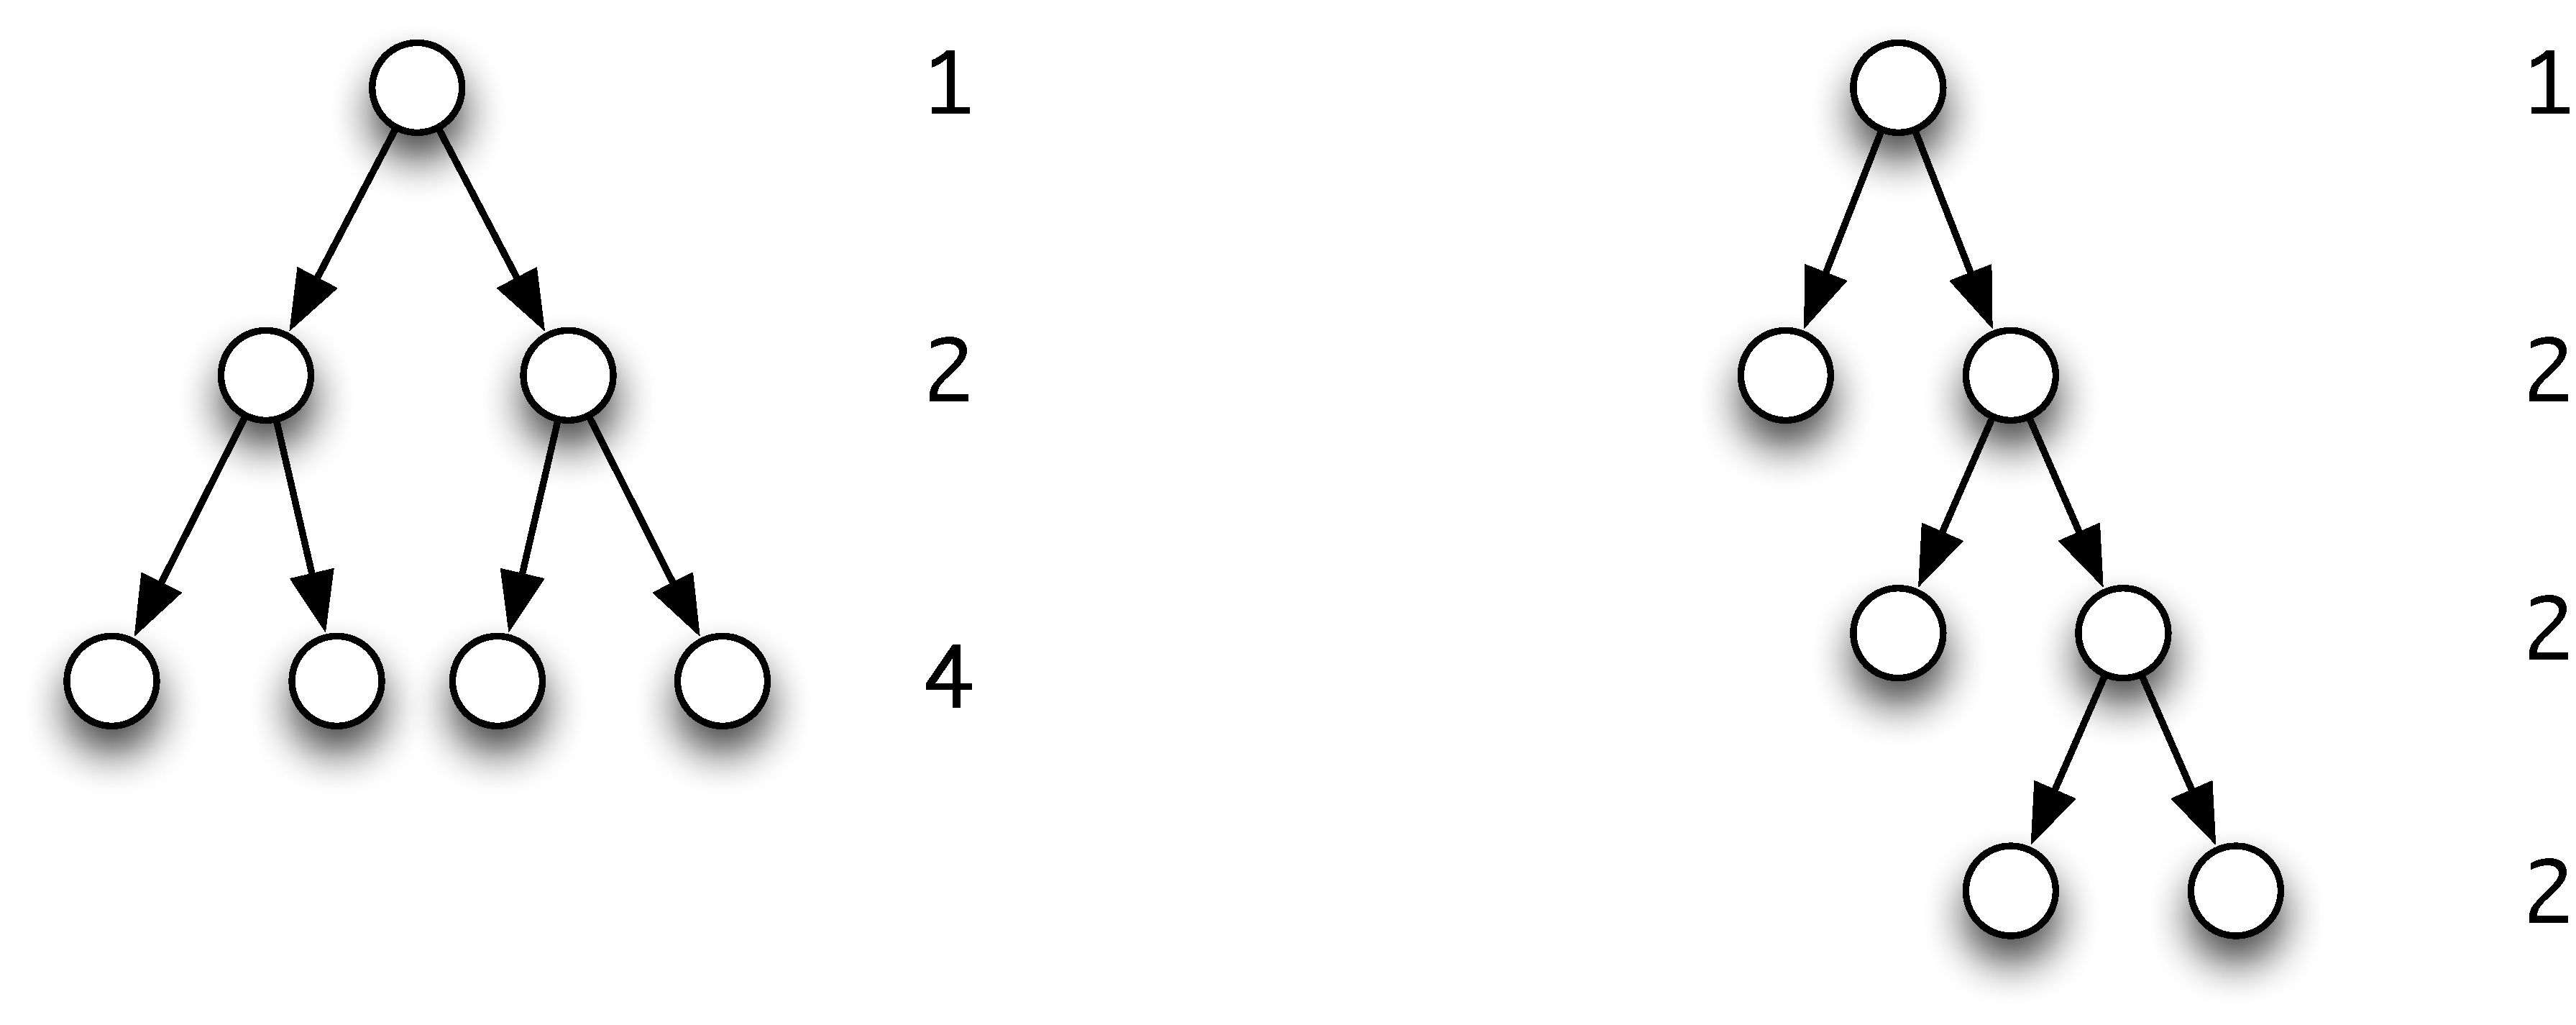
\includegraphics[width=3in]{Pictures/CountTrees.pdf}
\end{center}
\caption{Counting the number of nodes of trees.}
\label{countTrees}
\end{figure}
On the first level it has \texttt{1}, on the
second \texttt{2}, on the \texttt{k}th it has \texttt{2\up{(k-1)}}, so over all 
\texttt{b+1} levels it has
\begin{alltt}
1 + 2 + 4 + \ldots + 2\up{(k-1)} + \ldots + 2\up{b} = 2\up{(b+1)} - 1
\end{alltt}
as illustrated in Figure \ref{countTrees}.

We thus see that the size of a balanced tree is
\texttt{\Th(2\up{b})} in the length of the branches, \texttt{b}; taking logarithms, a
balanced tree of size \texttt{n} will therefore have branches of length 
\texttt{\Th(\ltwo\ n)} in the size of the tree. If a tree is not balanced, the
length of its longest branch can be of the same order as the size of the tree
itself; see Figure \ref{countTrees} for an example. 


\subexample*{3.}
Our final counting question concerns taking \textbf{sums}. If we are given one object
every day for \texttt{n} days, we have \texttt{n} at the end; if we are given 
\texttt{n} each day, we have \texttt{n\up{2}}; what if we are given \texttt{1} on the
first day, \texttt{2} on the second, and so on? What is the sum of the list 
\texttt{[1 ..\ n]}, in other words? Writing the list backwards, as well as forwards, we
have
\begin{alltt}
1     + 2     + 3     +  ...  + (n-1) + n +
n     + (n-1) + (n-2) +  ...  + 2     + 1 
\end{alltt}
adding {\em vertically\/} at each point we have a sum of \texttt{(n+1)}, 
\begin{alltt}
(n+1) + (n+1) + (n+1) +  ...  + (n+1) + (n+1)
\end{alltt}
and this
sum occurs \texttt{n} times, so 
\begin{alltt}
sum [1 ..\ n] = n*(n+1) `div` 2
\end{alltt}
which makes it 
\texttt{\Th(n\up{2})}, or quadratic. In a similar way, the sum of the squares is
\texttt{\Th(n\up{3})}, and so on.
 \end{example}


\begin{exercises}

\item
Show that the example
\begin{alltt}
f n = 2*n\up{2} + 4*n + 13
\end{alltt}
is \texttt{\Th(n\up{2})}.

\item
Give a table of the values of the functions \texttt{n\up{0}}, \texttt{log n}, 
\texttt{n\up{1}}, \texttt{n(log n)}, \texttt{n\up{2}}, \texttt{n\up{3}} and 
\texttt{2\up{n}} for the values 
\begin{alltt}
0 1 2 3 4 5 10 50 100 500 1000 10000 100000 10000000
\end{alltt}

\item
By giving the values of \texttt{d}, \texttt{m} and \texttt{c} (when necessary), show
that the following functions have the complexity indicated.
\begin{alltt}
f1 n = 0.1*n\up{5} + 31*n\up{3} + 1000              O(n\up{6})
f2 n = 0.7*n\up{5} + 13*n\up{2} + 1000              \Th(n\up{5})
\end{alltt}

\item
Show that \texttt{n\up{k} \lll\ 2\up{n}} for all positive \texttt{k}. By taking
logarithms of both sides, show that \texttt{log n \lll\ n\up{k}} for all
positive \texttt{k}.

\item
Show that 
\begin{alltt}
log \eqq\ ln \eqq\ \ltwo
\end{alltt}
and in fact that logarithms to any base have the same rate of growth.

\item
The function \texttt{fib} is defined by
\begin{alltt}
fib 0 = 0
fib 1 = 1
fib m = fib (m-2) + fib (m-1)
\end{alltt}
Show that \texttt{n\up{k}\ \lll\ fib n} for all \texttt{k}.

\item
Show that \texttt{\lll} is transitive -- that is \texttt{f\lll{}g} and 
\texttt{g\lll{}h} together imply that \texttt{f\lll{}h}. Show also that \texttt{\eqq} is an
equivalence relation.

\item
If \texttt{f} is \texttt{O(g)}, show that any constant multiple of \texttt{f} is also
of the same order. If \texttt{f1} and \texttt{f2} are \texttt{O(g)}, show that their
sum and difference are also \texttt{O(g)}. Are the same results valid
with \texttt{\Th} replacing \texttt{O}?

\item
If \texttt{f1} is \texttt{O(n\up{k1})} and \texttt{f2} is \texttt{O(n\up{k2})}, show
that their product,
\begin{alltt}
f n = f1 n * f2 n
\end{alltt}
is  \texttt{O(n\up{(k1+k2)})}.

\item
Prove by induction over the natural number \texttt{n} that
\begin{alltt}
1 + 2 + 4 + \ldots + 2\up{n} = 2\up{(n+1)} - 1
1 + 2 + \ldots + n      = n*(n+1) `div` 2
1\up{2} + 2\up{2} + \ldots + n\up{2}   = n*(n+1)*(2*n+1) `div` 6
1\up{3} + 2\up{3} + \ldots + n\up{3}   = (n*(n+1) `div` 2)\up{2}
\end{alltt}
\end{exercises}



\section{The complexity of calculations}
\label{complexCalc}

How can we measure the complexity of the functions we write? One answer is to
use an implementation of Haskell, which can be expected to produce some
diagnostic information about evaluation. We examine this option in Section \ref{foldingRev}, page \pageref{perfInPractice}, but for the moment we opt for a cleaner \emph{model} of what is going on, and we
choose to analyse the \emph{calculations} we have been using. There are
three principal measures we can use.
\begin{titemize}
\item The \textbf{time} taken to compute a result is given by the number
of steps in a calculation which uses lazy evaluation.
\index{behaviour!time}\index{complexity!time}
\item The \textbf{space} necessary for the computation can be
\index{behaviour!space}\index{complexity!space}
measured in two ways.
First, there is a lower limit on the amount of space we need for a calculation
to complete successfully. During calculation, the expression
being calculated grows and shrinks; obviously, we need enough
space to hold the {\em largest\/} expression built during the calculation.
This is often called the \textbf{residency}\index{residency} of the computation, we shall call
it the \textbf{space complexity}.
\item We can also make a measure of the
\textbf{total space} used by a computation, which in some way reflects the total
area of the calculation; it is of interest to implementers of functional
languages  but for users (and for us) the first two are the crucial measures.
\end{titemize}
How then do we measure the complexity of a function?

\subsection*{Complexity measures}

We measure the complexity of the function \texttt{f} by looking at the time and
space complexity as described above, as {\em functions\/} of the {\em size\/}
of the inputs to \texttt{f}. The size of a number is the number itself, while
the size of a list is given by its length, and of a tree by the number of
nodes it contains. We now look at a series of examples.
\begin{example}
\subexample*{1.}\index{complexity!\texttt{fac}}
Let us start with the example of \texttt{fac}.\minx{fac}
\begin{alltt}
fac :: Integer -> Integer
fac 0 = 1
fac n = n * fac (n-1)
\end{alltt}
Working through a calculation, we have
\begin{alltt}
fac n
\step n * fac (n-1)
\step ...
\step n * ((n-1) * ... * (2 * (1 * 1)) ...) \hfill (facMax)
\step n * ((n-1) * ... * (2 * 1) ...) 
\step n * ((n-1) * ... * 2 ...)  
\step ...
\step n!
\end{alltt}
The calculation contains \texttt{2*n+1} steps, and the largest expression, 
\texttt{(facMax)}, contains \texttt{n} multiplication symbols. This makes the time and
space complexity both \texttt{\Th(n\up{1})}, or linear.

\subexample*{2.}\index{complexity!\texttt{iSort}}
Next we look at insertion sort. Recall that
\begin{alltt}
iSort :: Ord a => [a] -> [a]

iSort []     = []\minx{iSort}
iSort (x:xs) = ins x (iSort xs)

ins x [] = [x]
ins x (y:ys) 
  | (x<=y)      = x:y:ys
  | otherwise   = y:ins x ys
\end{alltt}
A general calculation will be
\begin{alltt}
iSort [\aone,\atwo,\ldots,\subscr{a}{n-1},\subscr{a}{n}]
\step ins \aone\ (iSort [\atwo,\ldots,\subscr{a}{n-1},\subscr{a}{n}])
\step ...
\step ins \aone\ (ins \atwo\ ( ... (ins \subscr{a}{n-1}\ (ins \subscr{a}{n}\ []))...))
\end{alltt}
followed by the calculation of the \texttt{n} \texttt{ins}'s. 
What sort of behaviour does \texttt{ins} have? Take the general example of
\begin{alltt}
ins a [\aone,\atwo,\ldots,\subscr{a}{n-1},\subscr{a}{n}]
\end{alltt}
where we assume that \texttt{[\aone,\ldots,\subscr{a}{n}]} is sorted. There are
three possibilities:
\begin{titemize}
\item In the {\em best\/} case, when \texttt{a<=\aone}, the calculation takes
\texttt{1} step.
\item In the {\em worst\/} case, when \texttt{a>\subscr{a}{n}}, the calculation takes
\texttt{n} steps.
\item In an {\em average\/} case, the calculation will take \texttt{n/2} steps.
\end{titemize}
What does this mean for \texttt{iSort}? 
\begin{titemize}
\item In the {\em best\/} case, each \texttt{ins} will take one step, and the
calculation will therefore take a further \texttt{n} steps, making it 
\texttt{O(n\up{1})} in this case. 

\item On the other hand, in the {\em worst\/} case, the first \texttt{ins} will
take one step, the second two, and so on. By our counting argument in
Section \ref{funComplex} the calculation will take \texttt{O(n\up{2})} steps.

\item In an {\em average\/} case, the \texttt{ins}'s will take a total of
\begin{alltt}
1/2 + 2/2 + \ldots + (n-1)/2 + n/2
\end{alltt}
steps, whose sum is again \texttt{O(n\up{2})}, by our observation in
Section
\ref{counting} about the size of the sum \texttt{1+2...n}.
\end{titemize}
We therefore see that in most cases the algorithm takes quadratic time, but
in some exceptional cases, when sorting an (almost) sorted list, the
complexity is linear in the length of the list. In all cases the space usage
will also be linear. 


\subexample*{3.}\index{complexity!\texttt{++}}
Before looking at another sorting algorithm, we look at the time taken to
join together two lists, using \texttt{++}.\minx{++}
\begin{alltt}
[\aone,\atwo,\ldots,\subscr{a}{n-1},\subscr{a}{n}] ++ x
\step \aone : ([\atwo,\ldots,\subscr{a}{n-1},\subscr{a}{n}] ++ x)
\step \aone : (\atwo : [\subscr{a}{3},\ldots,\subscr{a}{n-1},\subscr{a}{n}] ++ x)
\step ... n-3 steps ...
\step \aone : (\atwo : \ldots\ : (\subscr{a}{n}:x)\ldots)
\end{alltt}
The time taken is {\em linear\/} in the length of the first list.

\subexample*{4.}\index{complexity!\texttt{qSort}}
Our second sorting algorithm, quicksort,\index{sorting!quicksort} is given by
\begin{alltt}
qSort :: Ord a => [a] -> [a]

qSort []     = []\minx{qSort}
qSort (x:xs) = qSort [z|z<-xs,z<=x] ++ [x] ++ qSort [z|z<-xs,z>x]
\end{alltt}
When the list is sorted and contains no duplicate elements, the calculation
goes thus:
\begin{alltt}
qSort [\aone,\atwo,\ldots,\subscr{a}{n-1},\subscr{a}{n}]
\step ... n steps ...
\step [] ++ [\aone] ++ qSort [\atwo,\ldots,\subscr{a}{n-1},\subscr{a}{n}] 
\step ... n-1 steps ...
\step \aone : ([] ++ [\atwo] ++ qSort [\subscr{a}{3},\ldots,\subscr{a}{n}])
\step ... n-2 steps ...
\step ...
\step \aone : (\atwo : (\subscr{a}{3} : \ldots\ \subscr{a}{n}:[])
\step [\aone,\atwo,\ldots,\subscr{a}{n-1},\subscr{a}{n}]
\end{alltt}
Since the number of steps here is {1+2+\ldots{}n}, we have \textbf{quadratic}
behaviour in this sorted case. In the {\em average\/} case, we split thus
\begin{alltt}
qSort [\aone,\atwo,\ldots,\subscr{a}{n-1},\subscr{a}{n}]
\step qSort [\subscr{b}{1},\ldots,\subscr{b}{n/2}] ++ [\aone] ++ qSort [\subscr{c}{1},\ldots,\subscr{c}{n/2}]
\end{alltt}
where the list has been bisected.
Forming the two sublists will take \texttt{O(n\up{1})} steps, as will the
joining together of the results. As we argued in Section \ref{funComplex},
there can be \texttt{\ltwo n} bisections before a list is reduced to one-element
lists, so we have \texttt{O(n\up{1})} steps to perform \texttt{O(log n)} many times;
this makes quicksort take \texttt{O(n(log n))} steps, {\em on average}, although we
saw that it can take quadratic steps in the worst (already sorted!)
case.\footnote{The explanation we have given here depends upon us
rearranging the order of the calculation steps; this is legitimate if we
observe that lazy evaluation of combinators is {\em optimal\/}, in the sense
of taking fewest steps to reach a result; any rearrangement can only give
more steps to our calculation, so the bound of \texttt{n(log n)} holds.}

The logarithmic behaviour here is characteristic of a `divide and conquer'
\index{divide and conquer}
algorithm: we split the problem into two smaller problems, solve these and
then recombine the results. The result is a comparatively efficient algorithm,
which reaches its base cases in \texttt{O(\ltwo\ n)} rather than \texttt{O(n\up{1})}
steps.

\end{example}
\begin{exercises}

\item
Estimate the time complexity of the two reverse functions given here:
\begin{alltt}
rev1 []     = []
rev1 (x:xs) = rev1 xs ++ [x]
\end{alltt}
and
\begin{alltt}
rev2            = shunt []
shunt xs []     = xs
shunt xs (y:ys) = shunt (y:xs) ys
\end{alltt}

\item
We can define multiplication by repeated addition as follows:
\begin{alltt}
mult n 0 = 0
mult n m = mult n (m-1) + n
\end{alltt}
`Russian' multiplication is defined by
\begin{alltt}
russ n 0 = 0
russ n m 
  | (m `mod` 2 == 0)    = russ (n+n) (m `div` 2)
  | otherwise           = russ (n+n) (m `div` 2) + n
\end{alltt}
Estimate the time complexity of these two multiplication algorithms.

\item
Estimate the time complexity of the Fibonacci function.

\item
Show that the worst-case time behaviour of the merge sort function below is
\texttt{O(n(log n))}.
\begin{alltt}
mSort :: Ord a => [a] -> [a]

mSort xs 
  | (len < 2)   = xs
  | otherwise   = mer (mSort (take m xs)) (mSort (drop m xs))
    where
    len = length xs
    m   = len `div` 2

mer :: Ord a => [a] -> [a]  -> [a]

mer (x:xs) (y:ys) 
  | (x<=y)      = x : mer xs (y:ys)
  | otherwise   = y : mer (x:xs) ys
mer (x:xs) []   = (x:xs)
mer []     ys   = ys
\end{alltt}
\index{complexity|)}
\end{exercises}
\section{Implementations of sets}
\index{sets!behaviour of implementations}


We first saw the \texttt{Set} abstract data
type in Section \ref{caseSets}, where we gave
an implementation based on ordered lists without repetitions. Alternatively
we can write an implementation based on arbitrary lists whose elements may
\index{lists!as sets}
occur in any order and be  repeated.
\begin{alltt}
type Set a = [a]\minx{Set}

empty        = []
memSet       = member
inter xs ys  = filter (member xs) ys
union        = (++)
subSet xs ys = and (map (member ys) xs)
eqSet xs ys  = subSet xs ys \&\& subSet ys xs
makeSet      = id
mapSet       = map
\end{alltt}
We can also write an implementation based on the search trees of Section
\index{search tree}
\ref{srchTrees}. We now compare the time complexity of these implementations,
and summarize the results in the table which follows.

\begin{center}
%\psframebox[framearc=0.1,linecolor=black,linewidth=0.5pt,framesep=0pt]
{\begin{tabular}{lccc}
\\[-9pt]
 & \ \ \  Lists\ \ \  &  Ordered lists &  Search trees\\
 &        &  &  (average) \\ 
\hline
\mi memSet & \mi O(n\up{1})  & \mi O(n\up{1}) & \mi O(log n) \\
\mi subSet & \mi O(n\up{2})  & \mi O(n\up{1}) & \mi O(n(log n)) \\
\mi inter & \mi O(n\up{2})  & \mi O(n\up{1}) & \mi O(n(log n)) \\
\mi makeSet & \mi O(n\up{0})  & \mi O(n(log n)) & \mi O(n(log n)) \\
\mi mapSet & \mi O(n\up{1})  & \mi O(n(log n)) & \mi O(n(log n)) \\[3pt]
\end{tabular}}
\end{center}


\noindent As we can see from the table, there is no clear `best' or `worst' choice;
\index{design!and behaviour}
depending upon the kind of set operation we intend to perform, different
implementations make more sense. This is one more reason for providing the
abstract data type\index{abstract data type}
boundary beneath which the implementation can be changed 
to suit the use to which the sets are being put without any need to change the user programs. Using a variant of search trees which are `balanced' so that all branches are of almost the same length, it is possible to achieve linear complexity for \texttt{subSet} and \texttt{inter} on average.


\begin{exercises}

\item
Confirm the time complexities given in the table above for the two list
implementations of sets.

\item
Implement the operations \texttt{subSet}, \texttt{inter}, \texttt{makeSet} and 
\texttt{mapSet} for the search tree implementation, and estimate the time complexity
of your implementations.

\item
Give an implementation of sets as lists without repetitions, and estimate
the time complexity of the functions in your implementation. 
\end{exercises}
\section{Space behaviour}
\label{spaceBeh}

A rule of thumb for estimating the space needed to calculate a result
is to measure the largest expression produced during the calculation. This is
accurate if the result being computed is a number or a Boolean, but it is
not when the result is a data structure, like a list.

\subsection*{Lazy evaluation}

Recall the explanation of lazy evaluation in Section \ref{lazyEval}, where
we explained that parts of results are printed as soon as possible. Once part
of a result is printed, it need no longer occupy any space. In estimating
space complexity, we must be aware of this.

Take the example of the lists \texttt{[m ..\ n]}, defined thus\minx{..}
\begin{alltt}
[m ..\ n] 
  | n>=m        = m:[m+1 ..\ n]
  | otherwise   = []
\end{alltt}
Calculating \texttt{[1 ..\ n]} gives
\begin{alltt}
[1 ..\ n]
      ?? n>=1
\step \underline{1}:[1+1 ..\ n]
      ??  n>=2
\step \underline{1}:[2 ..\ n]\index{underlining@\underline{underlining}}
\step \underline{1:2}:[2+1 ..\ n]
\step ...
\step \underline{1:2:3:...:n:[]}
\end{alltt}
where we have underlined those parts of the result which can be output. 
To measure the space complexity we look at the non-underlined part, which is
of constant size, so the space complexity is \texttt{O(n\up{0})}. The calculation
has approximately \texttt{2*n} steps, giving it linear time complexity, as
expected.

\subsection*{Saving values in {\latt where} clauses}
\index{behaviour!space!local definitions}

Consider the example of
\begin{alltt}
exam1 = [1 ..\ n] ++ [1 ..\ n]
\end{alltt}
The time taken to calculate this will be \texttt{O(n\up{1})}, and the space used
will be \texttt{O(n\up{0})}, but we will have to calculate the expression 
\texttt{[1 ..\ n]} {\em twice}. Suppose instead that we compute
\begin{alltt}
exam2 = list ++ list 
        where 
        list=[1 ..\ n]
\end{alltt}
The effect here is to compute the list \texttt{[1 ..\ n]} once, so that we save 
its value after calculating it in order to be able to
use it again. Unfortunately, this means that after
evaluating \texttt{list}, the whole of the list is stored, giving an 
\texttt{O(n\up{1})} space complexity.
 

This is a general phenomenon. If we save
something by referring to it in a \texttt{where} clause we have to pay
the penalty of the space that it occupies: if the space is available, fair
enough; if not, we have turned a working computation into one which fails for
lack of space.

This problem can be worse! Take the examples
\begin{alltt}
exam3 = [1 ..\ n] ++ [last [1 ..\ n]]
exam4 = list ++ [last list]
        where
        list=[1 ..\ n]
\end{alltt}
in which \texttt{last} returns the last element of a non-empty list.
The space required by \texttt{exam3} is \texttt{O(n\up{0})}, while in exam4 it is 
\texttt{O(n\up{1})}, since we hold on to the calculated value of \texttt{list} even
though we require only one value from it, the last. This feature, of keeping
hold of a large structure when we only need part of it, is called a
\textbf{space leak}\index{space leak}.
In the example here, the problem is clear, but in a larger
system the source of a space leak can be one of the most difficult debugging problems to solve.

The lesson of these examples must be that while it is {\em always\/} sensible
not to repeat the calculation of a simple value, saving a compound value
like a list or a tuple can increase the space usage of a program.

\subsection*{Saving space?}

As we saw in Section \ref{complexCalc}, the naive factorial function has 
\texttt{\index{factorial}
O(n\up{1})} space complexity, as it forms the expression
\begin{alltt}
n * ((n-1) * ... * (1 * 1)...)
\end{alltt}
before it is evaluated. Instead, we can perform the multiplications as we go
along, using
\begin{alltt}
newFac :: Integer -> Integer
newFac n = aFac n 1

aFac :: Integer -> Integer -> Integer
aFac 0 p = p
aFac n p = aFac (n-1) (p*n)
\end{alltt}
and compute the factorial of \texttt{n} using \texttt{aFac n 1}. Now, we examine
the calculation\index{factorial!complexity of}
\begin{alltt}
newFac n
\step aFac n 1
\step aFac (n-1) (1*n)
   ??  (n-1)==0 \step False
\step aFac (n-2) (1*n*(n-1))
\step ...
\step aFac 0 (1*n*(n-1)*(n-2)*...*2*1)
\step (1*n*(n-1)*(n-2)*...*2*1)\hfill (needVal)
\end{alltt}
so that the effect of this program is exactly the same: it still forms a large
unevaluated expression! The reason that the expression is unevaluated
is that it is not clear that its value is needed until the step \texttt{(needVal)}.

How can we overcome this? We ought to make the intermediate values 
{\em needed}, so that they are calculated earlier. We do this here by adding a test;
another method is given in Section \ref{foldingRev}.
\begin{alltt}
aFac n p 
  | p==p        = aFac (n-1) (p*n)
\end{alltt}
Now the calculation of the factorial of \texttt{4}, say, is
\begin{alltt}
aFac 4 1
\step aFac (4-1) (1*4)
    ??  (4-1)==0     \step False
    ??  (1*4)==(1*4) \step True \hfill (eqTest)
\step aFac (3-1) (4*3)
    ??  (3-1)==0     \step False
    ??  (4*3)==(4*3) \step True \hfill (eqTest)
\step aFac (2-1) (12*2)
\step ...
\step aFac 0 (24*1)
\step (24*1) 
\step  24
\end{alltt}
The lines \texttt{(eqTest)} show where the guard \texttt{p==p} is tested, and so
where the intermediate multiplications take place. From this we can conclude
that this version has better (constant) space behaviour. 

\begin{exercises}

\item
Estimate the space complexity of the function
\begin{alltt}
sumSquares :: Integer -> Integer
sumSquares n = sumList (map sq [1 ..\ n])
\end{alltt}
where
\begin{alltt}
sumList = foldr (+) 0
sq n    = n*n
\end{alltt}
and \texttt{map} and \texttt{[1 ..\ n]} have their standard definitions.

\item
Give an informal estimate of the complexity of the text processing functions
in Chapter \ref{defFunLists}. 

\end{exercises}





\section{Folding revisited}
\label{foldingRev}
\index{folding|(}

One of the patterns of computation which we identified in Chapter \ref{patternsGen}
is \textbf{folding} an operator or function into a list. This section
examines the complexity of the two standard folding functions, and
discusses how we can choose between them in program design. 
Before this we make a definition which expresses the fact of a function
needing to evaluate an argument. This distinction will be crucial to our full
understanding  of folding. 

\subsection*{Strictness}
\index{function!strict}
A function is \textbf{strict} in an
argument if the result is undefined whenever an undefined value is passed
to this argument. For instance, \texttt{(+)} is strict in both arguments,
while \texttt{(\&\&)} is strict in its first only. Recall that it is defined
by
\begin{alltt}
True  \&\& x = x
False \&\& x = False \hfill (andFalse)
\end{alltt}
The pattern match in the first argument forces it to be strict there, but
equation\break \texttt{(andFalse)} shows that it is possible to get an answer from 
\texttt{(\&\&)} when the second argument is \texttt{undef}, so it is therefore not
strict in the second argument. 

If a function is not strict in an argument, we say
that it is \textbf{non-strict} or \textbf{lazy} in that argument.
\index{function!lazy}

\subsection*{Folding from the right}
\index{foldr@\texttt{foldr}}
Our definition of folding was given by
\begin{alltt}
foldr :: (a -> b -> b) -> b -> [a] -> b

foldr f st []     = st
foldr f st (x:xs) = f x (foldr f st xs)
\end{alltt}
which we saw was of general application. Sorting a list, by insertion sort,
was given by
\begin{alltt}\minx{iSort}
iSort = foldr ins []
\end{alltt}
and indeed any primitive recursive definition over lists can be given by
applying \texttt{foldr}.

Writing the function applications as infix operations gives
\begin{alltt}
foldr f st [\aone,\atwo,\ldots,\subscr{a}{n-1},\subscr{a}{n}]
\step \aone\ `f` (\atwo\ `f` \ldots\ `f` (\subscr{a}{n-1} `f` (\subscr{a}{n} `f` st))\ldots)\hfill(foldr)
\end{alltt}
and shows why the `\textbf{r}' is added to the name:
bracketing is to the \textbf{r}ight, with the starting value \texttt{st} appearing to the
\textbf{r}ight of the elements also. If \texttt{f} is lazy in its second argument, we can
see from \texttt{(foldr)} that given the head of the list, output may be possible.
For instance, \texttt{map} can be defined like this
\begin{alltt}\index{map@\texttt{map}!defined using \texttt{foldr}}
map f = foldr ((:).f) []
\end{alltt}
and in calculating \texttt{map (+2) [1 ..\ n]}
we see
\begin{alltt}
foldr ((:).(+2)) [] [1 ..\ n]
\step ((:).(+2)) 1 (foldr ((:).(+2)) [] [2 ..\ n])
\step 1+2 : (foldr ((:).(+2)) [] [2 ..\ n])
\step \underline{3} : (foldr ((:).(+2)) [] [2 ..\ n])
\step ...
\end{alltt} 
As in Section \ref{spaceBeh}, we see that the space complexity of
this will be \texttt{O(n\up{0})},
since the elements of the list will be output as they are calculated. What
happens when we fold a strict operator into a list? The definition of \texttt{fac}
in Section \ref{complexCalc} can be rewritten as
\begin{alltt}
fac n = foldr (*) 1 [1 ..\ n]\minx{fac}
\end{alltt}
and we saw there that the effect was to give \texttt{O(n\up{1})} space
behaviour, since the multiplications in equation \texttt{(foldr)} cannot be
performed until the whole expression is formed, as they are bracketed to the
right. We therefore define a function to fold from the left.


\subsection*{Folding from the left}
Instead of folding from the right, we can define
\begin{alltt}\index{foldl@\texttt{foldl}}\index{foldl@\texttt{foldl}!type of}
foldl :: (a -> b -> a) -> a -> [b] -> a
foldl f st []     = st
foldl f st (x:xs) = foldl f (f st x) xs
\end{alltt} 
which gives
\begin{alltt}
foldl f st [\aone,\atwo,\ldots,\subscr{a}{n-1},\subscr{a}{n}]
\step (\ldots((st `f` \aone) `f` \atwo) `f` \ldots\ `f` \subscr{a}{n-1}) `f` \subscr{a}{n}\hfill(foldl)
\end{alltt}
We can calculate this in the factorial example, the effect being
\begin{alltt}
foldl (*) 1 [1 ..\ n]
\step foldl (*) (1*1) [2 ..\ n]
\step ...
\step foldl (*) (\ldots((1*1)*2)*\ldots*n) []
\step (\ldots((1*1)*2)*\ldots*n)
\end{alltt}
As in Section \ref{complexCalc}, the difficulty is that \texttt{foldl} as we have
defined it is not strict in its second argument. Using the standard function
\texttt{seq} \minx{seq}
\begin{alltt}
seq :: a -> b -> b
\end{alltt}
it is possible to make it strict in the second argument. The effect of
\texttt{seq x y} is to evaluate \texttt{x} before returning \texttt{y}. We can use
\texttt{seq} over any type, since it is a polymorphic function.
If we write
\begin{alltt}
strict :: (a -> b) -> a -> b
strict f x = seq x (f x)\minx{strict}
\end{alltt} 
then \texttt{strict f} is a \textbf{strict} version of the function \texttt{f} which
evaluates its argument \texttt{x} before computing the result \texttt{f x}.
We can therefore write a strict version of \texttt{foldl}, called
\texttt{foldl'},\index{foldl@\texttt{foldl\symbol{39}}!type of}
\begin{alltt}
foldl' :: (a -> b -> a) -> a -> [b] -> a\index{foldl@\texttt{foldl\symbol{39}}}
foldl' f st []     = st
foldl' f st (x:xs) = strict (foldl' f) (f st x) xs
\end{alltt} 
and this definition can be found in the \texttt{Data.List} module. Now, evaluating the example again,
\begin{alltt}
foldl' (*) 1 [1 ..\ n]
\step foldl' (*) 1 [2 ..\ n]
\step foldl' (*) 2 [3 ..\ n]
\step foldl' (*) 6 [4 ..\ n]
\step ...
\end{alltt}
Clearly, this evaluation is in constant space, \texttt{O(n\up{0})}. Can we draw
any conclusions from these examples?


\begin{figure}[t]
\begin{alltt}
module Main where

main = putStrLn (show (sumI 1 1000000))
-- main = putStrLn (show (sumIA 1 1000000))
-- main = putStrLn (show (sumIS 1 1000000))

sumI :: Integer -> Integer -> Integer
sumI n m
 | n>m       = 0
 | otherwise = n + sumI (n+1) m

sumIA :: Integer -> Integer -> Integer
sumIA n m = accIA n m 0

accIA n m s
 | n>m       = s
 | otherwise = accIA (n+1) m (n+s)

sumIS :: Integer -> Integer -> Integer
sumIS n m = accIS n m 0

accIS n m s
 | n>m       = s
 | otherwise = accIS (n+1) m $! (n+s)
\end{alltt}
\caption{Computing the sum \texttt{n+...+m}}
\label{sumDefs}
\end{figure}

\begin{figure}[t]
\begin{alltt}
./perfI.out +RTS -K100000000 -sstderr 
500000500000
     150,145,752 bytes allocated in the heap
      63,269,576 bytes copied during GC
      21,122,356 bytes maximum residency (7 sample(s))
      15,758,580 bytes maximum slop
              45 MB total memory in use (0 MB lost due to fragmentation)

  Generation 0:   217 collections,     0 parallel,  1.80s,  1.82s elapsed
  Generation 1:     7 collections,     0 parallel,  0.05s,  0.06s elapsed

  INIT  time    0.00s  (  0.00s elapsed)
  MUT   time    0.22s  (  0.24s elapsed)
  GC    time    1.86s  (  1.88s elapsed)
  EXIT  time    0.00s  (  0.00s elapsed)
  Total time    2.07s  (  2.12s elapsed)

  %GC time      89.6%  (88.5% elapsed)

  Alloc rate    695,428,301 bytes per MUT second

  Productivity  10.4% of total user, 10.2% of total elapsed
\end{alltt}
\caption{Performance of \texttt{ sumI 1 1000000}}
\label{perfIreport}
\end{figure}

\begin{figure}[t]
\begin{alltt}
./perfIS.out +RTS -K100000000 -sstderr 
500000500000
     126,083,156 bytes allocated in the heap
          27,444 bytes copied during GC
           5,340 bytes maximum residency (1 sample(s))
          11,044 bytes maximum slop
               1 MB total memory in use (0 MB lost due to fragmentation)

  Generation 0:   242 collections,     0 parallel,  0.00s,  0.00s elapsed
  Generation 1:     1 collections,     0 parallel,  0.00s,  0.00s elapsed

  INIT  time    0.00s  (  0.00s elapsed)
  MUT   time    0.16s  (  0.17s elapsed)
  GC    time    0.00s  (  0.00s elapsed)
  EXIT  time    0.00s  (  0.00s elapsed)
  Total time    0.16s  (  0.17s elapsed)

  %GC time       1.0%  (1.2% elapsed)

  Alloc rate    798,252,321 bytes per MUT second

  Productivity  98.7% of total user, 90.8% of total elapsed
\end{alltt}
\caption{Performance of \texttt{ sumIS 1 1000000}}
\label{perfISreport}
\end{figure}


\subsection*{Assessing performance in practice}\label{perfInPractice}
\index{performance!measurement in GHC|(}
\index{GHC!performance measurement|(}

We can get detailed performance information by \emph{compiling} programs using \texttt{ghc} and passing the right parameters to the executable program. For the simple examples here, we define the expressions we are interested in Figure \ref{sumDefs}.
This file is compiled using
\begin{alltt}
ghc Main.hs
\end{alltt}
and generates the executable file \texttt{a.out}, which we rename \texttt{perfI.out}, \texttt{perfIA.out} and \texttt{perfIS.out} to distinsguish the three different variants of the \texttt{main} program.

In the module we see three definitions of functions to sum integer ranges: \texttt{sumI}, a standard fold from the right, \texttt{sumIA}, a (lazy) fold from the left, and \texttt{sumIS} a \emph{strict} fold from the left. 

As we suggested earlier, we would only expect the last of the three to have reasonable behaviour, and indeed executing the compiled code for the first two gives this error message:
\begin{alltt}
Stack space overflow: current size 8388608 bytes.
Use `+RTS -Ksize -RTS' to increase it.
\end{alltt}
The brackets \texttt{+RTS ...\ -RTS} are used to pass parameters to the Haskell \emph{runtime system}. We can increase the stack size and gather post-mortem information using the flag \texttt{-sstderr} like this: 
\begin{alltt}
./perfI.out +RTS -K100000000 -sstderr -RTS
\end{alltt}
The report this produces is shown in Figure \ref{perfIreport}, which we explain now.
\begin{titemize}
\item
The first block of information explains how much memory has been used by the computation, and it is clear from this that the maximum space used -- the \emph{residency} -- is high.
\item
In the middle block we see the time devoted to various parts of the computation. \texttt{INIT} and \texttt{EXIT} explain the time to start and clean up, but the interesting results are \texttt{MUT} the \emph{mutation} time -- that is time actually computing -- and \texttt{GC}, which is time dealing with storage: recycling information that is not used, and copying information that is still in use. We can see from this that of the total time, 89.6\% is in \texttt{GC}, so we're doing something wrong here. \end{titemize}
The performance of \texttt{perfIA.out} is twice as bad (!), but for \texttt{perfIS.out}, as shown in  Figure \ref{perfISreport}, we see something much better. How do the two reports compare?
\begin{titemize}
\item
The mutation time for the two computations is similar for the two: 0.22 seconds for \texttt{sumI} and 0.16 for \texttt{sumIA}.
\item
On the other hand, the space behaviour is radically different. As we saw earlier, \texttt{GC} time for \texttt{sumI} is almost two seconds, whereas for \texttt{sumIA} it is negligible.
\end{titemize}
These reports give a clear indication of where problems can occur, and GHC has other facilities -- such as \emph{heap profiling} -- to help users to see where space is sued in a large system. The GHC documentation will tell you more.

\index{performance!measurement in GHC|)}
\index{GHC!performance measurement|)}



\subsection*{Designing folds}
\index{folding!designing folds}

When we fold in a {\em strict\/} function, we will form a list-sized
expression with \texttt{foldr}, so it will always be worth using \texttt{foldl'}.
This covers the examples of \texttt{(+)}, \texttt{(*)} and so forth. 

We saw earlier that when \texttt{map} was defined using \texttt{foldr} we could begin
to give output before the whole of the list argument was constructed. If we use
\texttt{foldl'} instead, we will have to traverse the whole list before giving any
output, since any \texttt{foldl'} computation follows the pattern
\begin{alltt}
foldl' f \subscr{st}{1} \subscr{xs}{1} 
\step foldl' f \subscr{st}{2} \subscr{xs}{2} 
\step ...
\step foldl' f \subscr{st}{k} \subscr{xs}{k} 
\step ...
\step foldl' f \subscr{st}{n} []
\step \subscr{st}{n}
\end{alltt}
so in the case of \texttt{map}, \texttt{foldr} is the clear
choice of the two.

A more interesting example is given by the function which is \texttt{True} only if
a list of Booleans consists of \texttt{True} throughout. We fold in \texttt{(\&\&)},
of
course, but should we use \texttt{foldr} or \texttt{foldl'}? The latter will give a
constant-space version, but will examine the {\em entire\/} list. Since 
\texttt{(\&\&)} is lazy in its second argument, we might not need to examine the value
returned from the remainder of the list. For instance,
\begin{alltt}
foldr (\&\&) True (map (==2) [2 ..\ n])
\step (2==2) \&\& (foldr (\&\&) True (map (==2) [3 ..\ n]))
\step True \&\& (foldr (\&\&) True (map (==2) [3 ..\ n]))
\step foldr (\&\&) True (map (==2) [3 ..\ n])
\step (3==2) \&\& (foldr (\&\&) True (map (==2) [4 ..\ n]))
\step False \&\& (foldr (\&\&) True (map (==2) [4 ..\ n]))
\step False
\end{alltt}
This version uses constant space, {\em and\/} may not examine the whole list;
\texttt{foldr} is therefore the best choice.

Beside the examples of \texttt{(+)} and \texttt{(*)}, there are many other 
examples where \texttt{foldl'} is preferable, including:
\begin{titemize}
\item Reversing a list. To use \texttt{foldr} we have to add an element \texttt{a} to
the end of a list, \texttt{x}. The operation \texttt{x++[a]} is strict in \texttt{x},
while the `cons' operation \texttt{(:)} is lazy in its list argument. 
\item
Converting a list of digits \texttt{"7364"} into a number is strict in both the
conversion of the front, \texttt{736} and the final character, \texttt{'4'}.
\end{titemize}
Since \texttt{foldl'} consumes an entire list before giving any output, it will
be of no use in defining functions to work over infinite lists or the partial
lists we looked at while writing interactive systems.

\begin{exercises}

\item
Define the functions to reverse a list and to convert a digit list into a
number using both \texttt{foldr} and \texttt{foldl'} and compare their behaviour 
by means of calculation.

\item
Is it better to define insertion sort using \texttt{foldr} or \texttt{foldl'}?
Justify your answer.

\item
How are the results of \texttt{foldr} and \texttt{foldl'} related? You may like to use
the functions \texttt{reverse} and \texttt{flip} in framing your
answer.

\item
What is the relationship between \texttt{foldr} and \texttt{foldl'} when the
function to be folded is

\[\begin{tabular}{ll}
associative: &  \texttt{a `f` (b `f` c) = (a `f` b) `f` c};\\
has \texttt{st} as an identity: &  \texttt{st `f` a = a = a `f` st};\\
commutative: &  \texttt{a `f` b = b `f` a};
\end{tabular}
\]
and what is the relationship when all three hold?

\index{folding|)}

\end{exercises}

\begin{figure}[t]\begin{alltt}
fibP 3
= (y,x+y)
  where
  (x,y) = fibP 2
        = (\subscr{y}{1},\subscr{x}{1}+\subscr{y}{1})
          where
          (\subscr{x}{1},\subscr{y}{1}) = fibP 1
                  = (\subscr{y}{2},\subscr{x}{2}+\subscr{y}{2})
                    where
                    (\subscr{x}{2},\subscr{y}{2}) = fibP 0
                 \vertline{30pt}          = (0,1)
       \vertline{78pt}          = (1,1)
\vertline{126pt}        = (1,2)
= (2,3)
\end{alltt}
\caption{Calculating \texttt{fibP 3}.}
\label{fibCalc}
\end{figure}



\section{Avoiding recomputation: memoization}
\index{memoization|(}

In this section we look at general strategies which allow us to
avoid having  to
recompute results during the course of evaluating an expression. This
happens particularly in some recursive solutions of problems, where the
solutions to sub-problems can be used repeatedly.

We begin the discussion by looking again at the Fibonacci function.
\index{Fibonacci numbers}
\begin{alltt}
fib :: Integer -> Integer
fib 0 = 0
fib 1 = 1
fib n = fib (n-2) + fib (n-1)
\end{alltt}
This definition is remarkably inefficient. Computing \texttt{fib n} calls 
\texttt{fib (n-2)} and \texttt{fib (n-1)} -- the latter will call \texttt{fib (n-2)} again,
and
within {\em each\/} call of \texttt{fib (n-2)} there will be two calls to \texttt{fib
(n-3)}. The time complexity of \texttt{fib} is greater than any power. How might
we avoid this recomputation? We explore two ways of augmenting the definition
to make it efficient; in the first we return a complex data structure from
each call, and in the second we define an infinite list to hold all the values
of the function.

First we observe that to get the value at \texttt{n} we need the two
previous values; we could therefore return {\em both\/} these
values in the result.
\begin{alltt}\minx{fibP}
fibP :: Integer -> (Integer,Integer)
fibP 0 = (0,1)
fibP n = (y,x+y)
         where
         (x,y) = fibP (n-1)
\end{alltt}
A calculation is given in Figure \ref{fibCalc}, where different variables 
\texttt{\subscr{x}{1}}, \texttt{\subscr{y}{1}}\index{variable}
and so on have been used for the different occurrences of the local
variables \texttt{x} and \texttt{y}; this is not necessary  but does make the
different occurrences clearer.

As an alternative strategy, we can try to define the list of Fibonacci values,
\texttt{fibs},  directly. The values of the \texttt{fib} function given above now become
values at particular indices:
\begin{alltt}
fibs      :: [Integer]
fibs!!0     = 0
fibs!!1     = 1
fibs!!(n+2) = fibs!!n + fibs!!(n+1)
\end{alltt}
This gives a {\em description\/} of the list, but it is not executable in this
form. The first two lines tell us that \texttt{fibs = 0 :\ 1 :\ rest}, while the
third equation tells us what the \texttt{rest} is. The \texttt{(n+2)}nd element of
\texttt{fibs} is the \texttt{n}th element of \texttt{rest}; similarly, the \texttt{(n+1)}st
element is the \texttt{n}th element of \texttt{(tail fibs)}. We therefore have, for
every \texttt{n}, 
\begin{alltt}
rest!!n = fibs!!n + (tail fibs)!!n
\end{alltt}
which says that each element is got by adding the corresponding elements of
two lists, that is
\begin{alltt}
rest = zipWith (+) fibs (tail fibs)
\end{alltt}
so that putting the parts together, we have
\begin{alltt}
fibs ::[Integer]\minx{fibs}
fibs = 0 : 1 : zipWith (+) fibs (tail fibs)
\end{alltt}
a \textbf{process network}\index{lists!as processes}
computing the Fibonacci numbers. This gives a linear
time, constant space algorithm for the problem, in contrast to the pair
solution which is linear in both time and space, since all the nested calls to
\texttt{fibP} are built before any result can be given.

\subsection*{Dynamic programming}
\index{dynamic programming|(}

\begin{figure}[t]\begin{alltt}\minx{mLen}\minx{maxLen}\minx{maxTab}
mLen :: Eq a => [a] -> [a] -> Integer

mLen xs []        = 0
mLen [] ys        = 0
mLen (x:xs) (y:ys) 
  | x==y        = 1 + mLen xs ys
  | otherwise   = max (mLen xs (y:ys)) (mLen (x:xs) ys)

maxLen :: Eq a => [a] -> [a] -> Int -> Int -> Int

maxLen xs ys 0 j = 0 \hfill(maxLen.1)
maxLen xs ys i 0 = 0\hfill(maxLen.2)
maxLen xs ys i j
  | xs!!(i-1) == ys!!(j-1)  
     = (maxLen xs ys (i-1) (j-1)) + 1  \hfill(maxLen.3)
  | otherwise              
     = max (maxLen xs ys i (j-1)) (maxLen xs ys (i-1) j) \hfill(maxLen.4)

maxTab ::  Eq a => [a] -> [a] -> [[Int]]

maxTab xs ys
  = result
    where 
    result = [0,0 ..\ ] : zipWith f [0 ..\ ] result
    f i prev  
        = ans
          where
          ans   = 0 : zipWith g [0 ..\ ] ans
          g j v 
            | xs!!i == ys!!j      = prev!!j + 1
            | otherwise           = max v (prev!!(j+1))
\end{alltt}
\caption{Three algorithms for the maximum common subsequence.}
\label{maxSubFig}
\end{figure}

The example in this section illustrates a general method of solving problems
by what is known as \textbf{dynamic programming}. Dynamic programming
solutions work by breaking a problem into subproblems but, as in the
Fibonacci example, the subproblems will not be independent, in general. A
naive solution therefore will contain massive redundancy, which we remove by
building a  {\em table\/} of solutions to subproblems.

The example we consider is to find the length of a \textbf{maximal
common subsequence}
\index{maximal common subsequence}
of two lists -- the subsequences need not have all their elements adjacent.
In the examples of
\begin{alltt}
[2,1,4,5,2,3,5,2,4,3]      [1,7,5,3,2]
\end{alltt}
the length of \texttt{4} is given by the subsequence \texttt{[1,5,3,2]}. This
problem is not simply a `toy'; a solution to this can be used to find the
common lines in two files, which gives the basis of the Unix \texttt{diff}
\minx{diff}
program, which is used, for instance, for comparing different versions of
programs stored in separate files. 


The naive
solution is given by \texttt{mLen} in Figure \ref{maxSubFig}. The interesting
part of the definition is given by the third equation. In the case where the
lists have equal first elements, these elements must be in
a maximal common subsequence, so we find the overall solution by looking in the
tails  and adding one to the result. More problematic is the case in which the
heads are distinct. We have the choice of excluding either \texttt{x} or \texttt{y}; in
this algorithm we try both possibilities  and take the maximal result. There, of
course, is the source of the redundant computations -- each of these may well
give rise to a computation of \texttt{mLen xs ys}. How are we to avoid this
situation? We shall store these results in a \textbf{table}, which 
will be represented by
a list of lists. Once a result appears in the table, we have no need
to recompute it.

As
an intermediate step, we rewrite the solution as \texttt{maxLen} which uses list
indexing, so that 
\begin{alltt}
maxLen xs ys u v
\end{alltt}
is the longest common subsequence in the lists \texttt{take u xs} and \texttt{take v
ys}. The function is given in Figure \ref{maxSubFig}, and the definition is a
straightforward adaptation of \texttt{mLen}.

Now we aim to define the table \texttt{maxTab xs ys} so that 
\begin{alltt}
(maxTab xs ys)!!u!!v = maxLen xs ys u v
\end{alltt}
This requirement is made specific by equations \texttt{(maxLen.1)} to \texttt{(maxLen.4)}. The
base case is given by \texttt{(maxLen.1)}, stating that
\begin{alltt}
(maxTab xs ys)!!0!!v = 0
\end{alltt}
for all \texttt{v}. In other words,
\begin{alltt}
(maxTab xs ys)!!0 = [0,0 ..\ ]
\end{alltt}
so,
\begin{alltt}
result = [0,0 ..\ ] :  ...
\end{alltt}
The equations \texttt{(maxLen.2)} to \texttt{(maxLen.4)} tell us how to define the list 
\texttt{maxTab!!(i+1)} from the list \texttt{maxTab!!i}, and i, so we can define
\begin{alltt}
maxTab xs ys = result
               where
               result = [0,0 ..\ ] : zipWith f [0 ..\ ] result
\end{alltt}
where \texttt{f ::\ Integer -> [Integer] -> [Integer]} is the function taking \texttt{i} and
the previous value, \texttt{maxTab!!i}, to \texttt{maxTab!!(i+1)}. Now we have to define
this latter, which appears in the solution as \texttt{ans}. 

Equation \texttt{(maxLen.2)} tells  us that it starts with \texttt{0}, and \texttt{g} is the
function taking \texttt{maxTab!!(i+1)!!j} and \texttt{j} to \texttt{maxTab!!(i+1)!!(j+1)}, where
we are also able to use the values of \texttt{maxTab!!i}, named by \texttt{prev}.
Using these insights, the definition of \texttt{g} is a straightforward
transliteration of \texttt{(maxLen.3)} and \texttt{(maxLen.4)}:
\begin{alltt}
ans   = 0 : zipWith g [0 ..\ ] ans
g j v 
  | xs!!i == ys!!j      = prev!!j + 1
  | otherwise           = max v (prev!!(j+1))
\end{alltt}
The top-level result is given by calling 
\begin{alltt}
maxTab xs ys !! (length xs) !! (length ys)
\end{alltt}
and this is computed in linear time and space.

Haskell provides arrays which can be used to give a more efficient implementation of a
number of algorithms, including this one here. Further details can
be found in the library module \texttt{Array.hs}\minx{Array.hs} and its documentation.

\index{dynamic programming|)}

\subsection*{Greedy algorithms}
\index{greedy algorithm}

A greedy solution to a dynamic programming problem works by building up the
optimal solution by making {\em local\/} choices of what appear to be the
best solutions of sub-problems. In the common subsequence problem, we can 
think of searching along the two lists in a single sweep, looking
successively for the first points of agreement; we search all pairs of indices
smaller than \texttt{n} before looking at \texttt{n}.  
In an example, the greedy
solution gives 
\begin{center}
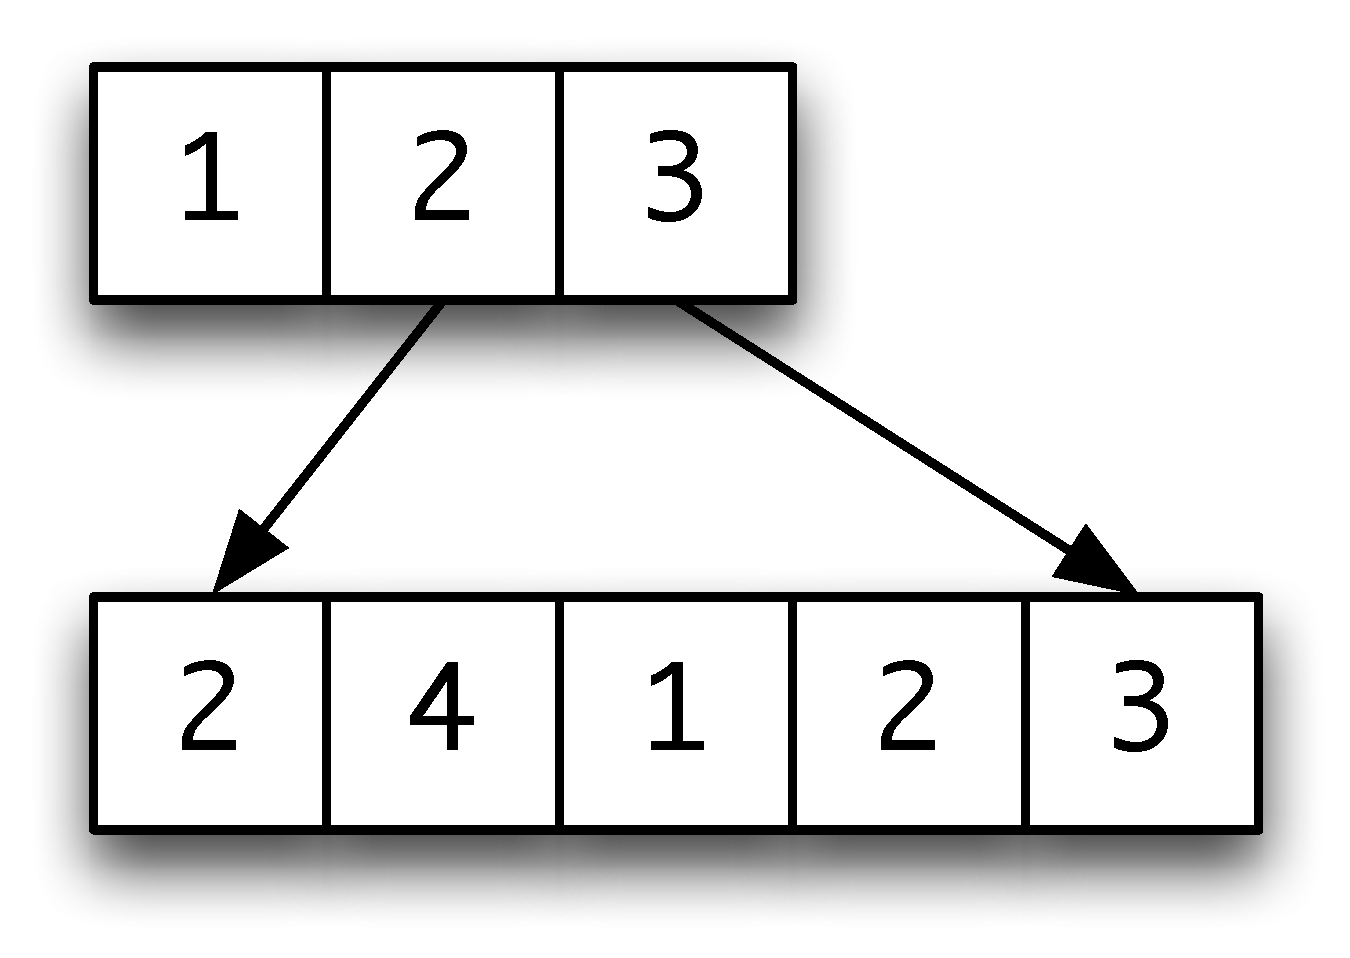
\includegraphics[width=1.7in]{Pictures/Greedy.pdf}
\end{center}
which is {\em not\/} optimal: the subsequence \texttt{[1,2,3]} has been missed,
since we make the choice of \texttt{2} the first element,  it is the first
point of agreement. This local choice is not part of an optimal global
solution, but the algorithm gives reasonable performance. 

In many situations, where local choices are always part of a global
solution, a greedy solution will work. Examples we have seen thus far include
\begin{titemize}
\item the line-splitting algorithm we gave in Chapter \ref{defFunLists} is optimal
in minimizing the sum of the inter-word spaces when the
lines are justified;
\index{text processing}
\item the Huffman codes described in Chapter \ref{codes} are optimal in the
sense of giving the shortest possible codings of files. We did not search all
possible sets of codes in giving the Huffman code, rather we built it up from
locally sensible choices. 
\index{Huffman codes}
\end{titemize}

\begin{exercises}

\item
Give an implementation of the greedy solution to the maximal common
subsequence problem, and show that it behaves as explained above on the
lists \texttt{[1,2,3]} and \texttt{[2,4,1,2,3]} above.

\item
Can you give an improvement of the maximal common subsequence solution along
the lines of \texttt{fibP}, returning a complex (finite) data structure as the
result of a function call, rather than simply one value?

\item
Finding the `edit distance' between two strings was first discussed in
Section  \ref{algDesign} where we gave a dynamic programming solution to the
problem. Show how you can give an efficient implementation of this
algorithm using the techniques of this section, and also how you give a greedy
solution to the problem. How do the two solutions compare? 

\item
Based on the examples of this section, provide a program which gives the
difference between two files, matching the corresponding lines  and giving the
output in a suitable form, such as a list of the pairs of matching line
numbers  or a form copied from the Unix \texttt{diff} program.
\end{exercises}

\begin{summary}
In this chapter we have examined the efficiency of lazy functional
programs. We saw that we are able to analyse the time
complexity of many of our more straightforward
functions without too much difficulty. To analyse
the space behaviour is more difficult, but we have shown how the space
consumption of lazy programs can be estimated from our calculations.

The introduction of \texttt{foldl} brings the space issue into focus, and the
distinction we made between strict and lazy functions allows us to
analyse the different behaviour of the two folds.

We concluded the discussion with an application of lazy infinite lists to 
memoizing results for reuse; the transition from naive to
efficient was done in a systematic way, which can be carried over to other
application areas. 

This chapter has provided an introduction to the study of functional
program behaviour; much more information -- particularly about
functional data structures -- can be found in \citeN{okasakiBook}.
\end{summary}

 
\index{behaviour|)}
\index{memoization|)}




%\end{document}
